\documentclass[11pt,a4paper]{article}

% -----------------------------------------------------------------------
% Packages
% -----------------------------------------------------------------------
\usepackage[T1]{fontenc}
\usepackage[utf8]{inputenc}
\usepackage{lmodern}
\usepackage{microtype}
\usepackage{geometry}
\geometry{a4paper, margin=2.5cm}

\usepackage{amsmath,amssymb}
\usepackage{booktabs}
\usepackage{array}
\usepackage{tabularx}
\usepackage{multirow}
\usepackage{graphicx}
\usepackage{tikz}
\usetikzlibrary{shapes.geometric, arrows.meta, positioning, fit, backgrounds}
\usepackage{xcolor}
\usepackage{hyperref}
\hypersetup{
    colorlinks=true,
    linkcolor=blue!60!black,
    citecolor=blue!60!black,
    urlcolor=blue!60!black
}
\usepackage{cleveref}
\usepackage{natbib}
\bibliographystyle{abbrvnat}
\setcitestyle{authoryear,open={(},close={)}}

\usepackage{abstract}
\renewcommand{\abstractnamefont}{\normalfont\bfseries}

\usepackage{titlesec}
\titleformat{\section}{\large\bfseries}{\thesection}{1em}{}
\titleformat{\subsection}{\normalsize\bfseries}{\thesubsection}{1em}{}

\usepackage{enumitem}
\usepackage{parskip}
\setlength{\parskip}{4pt}

% -----------------------------------------------------------------------
% Custom colours
% -----------------------------------------------------------------------
\definecolor{vatsa-blue}{RGB}{30,80,160}
\definecolor{vatsa-gray}{RGB}{100,100,100}
\definecolor{modgreen}{RGB}{0,130,80}
\definecolor{modred}{RGB}{180,30,30}

% -----------------------------------------------------------------------
% Title block
% -----------------------------------------------------------------------
\title{%
  \vspace{-1em}
  {\large\textcolor{vatsa-gray}{Preprint --- Version 1.0 \quad April 2026}}\\[0.6em]
  {\LARGE\bfseries VATSA: Video, Audio, Text, Sensory, Action}\\[0.3em]
  {\large A Unified Five-Modality Architecture for\\
   Human-Level Perception and Action}
}

\author{%
  \textbf{Vinay Kumar K V}\\[0.3em]
  DBA Candidate in AI \& ML, Walsh College (2025--2028)\\
  PGP in AI \& ML, Texas McCombs School of Business (2025--2026)\\
  London, United Kingdom\\[0.4em]
  \href{https://github.com/vinaykumarkv/VATSA}{\texttt{github.com/vinaykumarkv/VATSA}}
}

\date{%
  April 2026\quad(Preprint --- Version 1.0)\\[0.3em]
  \small\textcolor{vatsa-gray}{%
    DOI:~\href{https://doi.org/10.5281/zenodo.19714353}%
    {\texttt{10.5281/zenodo.19714353}}
  }%
}

% -----------------------------------------------------------------------
\begin{document}
% -----------------------------------------------------------------------

\maketitle
\thispagestyle{empty}

\begin{abstract}
We present \textbf{VATSA} (Video, Audio, Text, Sensory, Action), a proposed unified
architecture for human-level multimodal AI that integrates five distinct perceptual
and actuation streams within a single coherent framework.  While state-of-the-art
multimodal models such as GPT-4o \citep{openai2024gpt4o}, Gemini Ultra, and
Uni-MoE \citep{li2024unimoe} span two to four modalities, no existing system jointly
addresses video, audio, text, physiological/IoT sensory data, and grounded action.
Recent survey work on unified multimodal understanding \citep{yang2025survey}
explicitly identifies the absence of sensory integration and closed-loop action as
critical open frontiers.

VATSA addresses these gaps through four architectural principles:
(1)~a \emph{shared latent space} in which all modality encoders project into a common
high-dimensional embedding;
(2)~\emph{cross-modal attention} enabling dynamic inter-modality interaction at the
representation level;
(3)~a \emph{temporal coherence layer} that synchronises streams with heterogeneous
sampling rates; and
(4)~a \emph{closed-loop action head} supporting physical, digital, and communicative
outputs.

We present the conceptual architecture, motivating applications in healthcare,
regulated pharmaceutical environments, autonomous systems, and adaptive education,
an analysis of open research questions, and a phased implementation roadmap
(2026--2028).  This paper constitutes a timestamped declaration of the architectural
hypothesis, providing a foundation for systematic empirical validation as each modality
module is built and published openly.  Benchmarks and experimental results will be
incorporated in subsequent revisions.

\medskip
\noindent\textbf{Keywords:} multimodal learning, unified architecture, cross-modal
attention, sensory fusion, embodied AI, vision-language-action models
\end{abstract}

\newpage
\tableofcontents
\newpage

% =========================================================================
\section{Introduction}
\label{sec:intro}
% =========================================================================

Human intelligence is fundamentally multimodal.  A clinician assessing a patient does
not read a chart alone --- they listen to the patient speak, observe facial expression
and gait, monitor vital signs from sensors, and simultaneously formulate and execute
a treatment plan.  This seamless, context-aware fusion of multiple perceptual streams
with grounded action is the hallmark of human-level cognition, and it remains largely
unrealised in artificial systems.

Contemporary AI has made spectacular progress within individual modalities.  Large
language models \citep{vaswani2017attention} exhibit remarkable language
understanding; vision-language models \citep{radford2021clip,alayrac2022flamingo}
fuse image and text; speech models handle audio; and vision-language-action (VLA)
models \citep{ma2024vla} begin to integrate perception with robotic control.  Yet even
the most capable multimodal systems today address at most three or four modalities in a
unified way, and none integrates physiological or IoT sensory streams alongside
language, audio, video, and action within a single architecture.

\textbf{VATSA} (Video, Audio, Text, Sensory, Action) is a proposed architecture
designed to fill this gap.  It is motivated by a core claim: \emph{five modalities, not
two or three, are required to replicate the breadth of human sensorimotor
intelligence}.  The five streams are:

\begin{itemize}[leftmargin=2em]
  \item \textbf{Video} --- spatial and temporal scene understanding
  \item \textbf{Audio} --- speech, sound events, prosody, environmental audio
  \item \textbf{Text}  --- language understanding, reasoning, instruction following
  \item \textbf{Sensory} --- physiological signals, IoT sensors, proprioception
  \item \textbf{Action} --- closed-loop physical or digital output
\end{itemize}

This paper presents the conceptual architecture of VATSA, its relationship to existing
work, motivating application domains, open research questions, and the phased
implementation roadmap through which it will be empirically tested.  The repository
hosting all associated code and documentation is publicly available at
\url{https://github.com/vinaykumarkv/VATSA}.

\paragraph{Scope of this preprint.}
This is a concept and roadmap paper.  It does not report experimental results; those will
be incorporated as each phase of the roadmap is completed.  The purpose of early
publication is to establish a timestamped, peer-visible record of the architectural
hypothesis and to invite community engagement, critique, and collaboration from the
outset.

% =========================================================================
\section{Background and Related Work}
\label{sec:related}
% =========================================================================

\subsection{Multimodal Foundation Models}

The past four years have seen a rapid convergence of modalities within foundation
models.  CLIP \citep{radford2021clip} demonstrated powerful vision-language alignment
via contrastive learning.  Flamingo \citep{alayrac2022flamingo} introduced few-shot
visual language models.  GPT-4o \citep{openai2024gpt4o} extended this to audio,
supporting real-time speech interaction alongside vision and text.  Gemini Ultra
similarly unifies three modalities.  Uni-MoE \citep{li2024unimoe} employs
Mixture-of-Experts (MoE) routing across four modalities (video, audio, image, text),
representing the most comprehensive publicly described architecture to date.

Crucially, \citet{yang2025survey} conducted a comprehensive survey of 700+ papers on
unified multimodal understanding and generation, and explicitly identifies two
outstanding frontiers: (1)~the integration of physiological and IoT sensory data, and
(2)~action grounding within a unified architecture.  VATSA addresses both
simultaneously.

\subsection{Shared Latent Space Modelling}

ShaLa \citep{cui2025shala} proposes multimodal shared latent space modelling via
diffusion, demonstrating that a common embedding space can support cross-modal
generation and alignment beyond vision-language pairs.  VATSA extends this principle
across five modalities, treating the shared latent space as the central representational
substrate.

\subsection{Embodied AI and Vision-Language-Action Models}

\citet{ma2024vla} provide the first comprehensive taxonomy of vision-language-action
(VLA) models, covering architectures that ground language and vision in physical
robotic action.  \citet{liu2025embodied} survey the broader landscape of embodied AI,
identifying temporal alignment across heterogeneous sensing modalities as an open
challenge.  VATSA incorporates an action head directly into the unified architecture,
extending VLA principles to include audio and sensory streams.

\subsection{Generalist Agents}

Gato \citep{reed2022gato} demonstrated that a single transformer can be trained across
diverse tasks spanning text, images, and robotic control, establishing the viability of
truly generalist architectures.  VATSA builds on this spirit while focusing specifically
on the five modalities most relevant to human-environment interaction.

\subsection{The Modality Gap}

\Cref{tab:modality} summarises the modality coverage of leading models.  No existing
published architecture covers all five VATSA modalities.

\begin{table}[ht]
\centering
\caption{Modality coverage of leading multimodal models.
  \checkmark~=~supported;\; $\sim$~=~partial;\; $\times$~=~not supported.}
\label{tab:modality}
\renewcommand{\arraystretch}{1.25}
\begin{tabular}{lcccccc}
\toprule
\textbf{Model} & \textbf{Video} & \textbf{Audio} & \textbf{Text}
               & \textbf{Sensory} & \textbf{Action} & \textbf{\# Mod.}\\
\midrule
GPT-4o \citep{openai2024gpt4o}          & $\sim$       & \checkmark & \checkmark & $\times$    & $\times$    & 3 \\
Gemini Ultra (Google, 2023)              & \checkmark   & \checkmark & \checkmark & $\times$    & $\times$    & 3 \\
LLaVA / LLaMA 3.2                       & \checkmark   & $\times$   & \checkmark & $\times$    & $\times$    & 2 \\
Gato \citep{reed2022gato}               & $\sim$       & $\times$   & \checkmark & $\sim$      & \checkmark  & 3--4 \\
Uni-MoE \citep{li2024unimoe}            & \checkmark   & \checkmark & \checkmark & $\times$    & $\times$    & 4 \\
AudioPaLM \citep{barrault2023audiopalm} & $\times$     & \checkmark & \checkmark & $\times$    & $\times$    & 2 \\
\midrule
\textbf{VATSA (proposed)}               & \checkmark   & \checkmark & \checkmark & \checkmark  & \checkmark  & \textbf{5} \\
\bottomrule
\end{tabular}
\end{table}

% =========================================================================
\section{The VATSA Architecture}
\label{sec:arch}
% =========================================================================

VATSA is built on four interconnected architectural principles.
\Cref{fig:arch} provides a schematic overview.

% ------------------------------------------------------------------
%  Architecture diagram (TikZ) — vertical layout, guaranteed page-fit
% ------------------------------------------------------------------
\begin{figure}[ht]
\centering
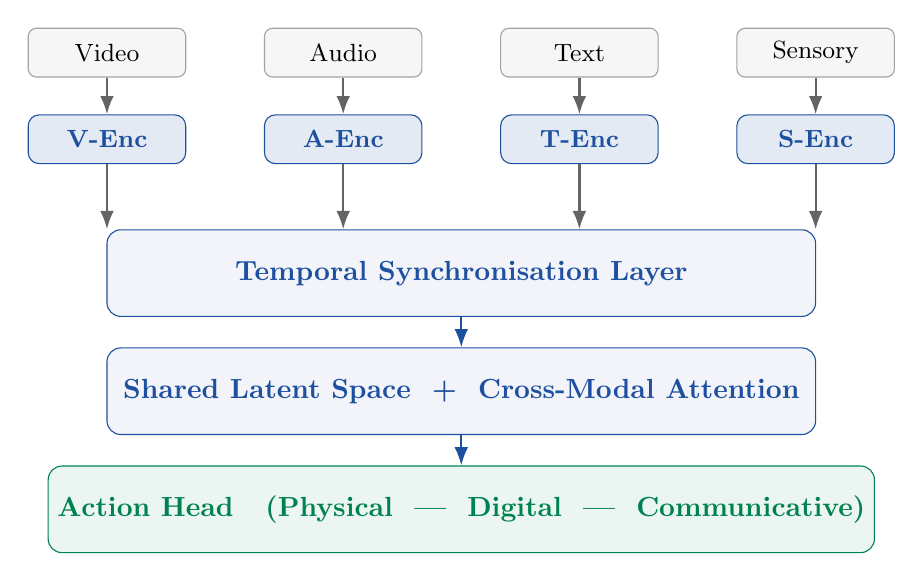
\begin{tikzpicture}[
    node distance = 0.45cm and 1.4cm,
    %% Modality input label
    mod/.style  = {rectangle, rounded corners=3pt,
                   draw=vatsa-gray!60, fill=gray!7,
                   minimum width=2.0cm, minimum height=0.62cm,
                   font=\small, align=center},
    %% Encoder box
    enc/.style  = {rectangle, rounded corners=4pt,
                   draw=vatsa-blue, fill=vatsa-blue!12,
                   minimum width=2.0cm, minimum height=0.62cm,
                   font=\small\bfseries, text=vatsa-blue, align=center},
    %% Wide processing box (full width, centred)
    wbox/.style = {rectangle, rounded corners=5pt,
                   draw=vatsa-blue, fill=vatsa-blue!6,
                   minimum width=9.0cm, minimum height=1.1cm,
                   font=\normalsize\bfseries, text=vatsa-blue, align=center},
    %% Action head box
    abox/.style = {rectangle, rounded corners=5pt,
                   draw=modgreen, fill=modgreen!8,
                   minimum width=9.0cm, minimum height=1.1cm,
                   font=\normalsize\bfseries, text=modgreen, align=center},
    arr/.style  = {-Latex, thick, color=vatsa-gray},
    darr/.style = {-Latex, thick, color=vatsa-blue},
]

%% ---- Row 1: four modality pairs side by side ----
\node[mod] (video)   at (0,    0) {Video};
\node[enc] (venc)    at (0,   -1.1) {V-Enc};

\node[mod] (audio)   at (3.0,  0) {Audio};
\node[enc] (aenc)    at (3.0, -1.1) {A-Enc};

\node[mod] (text)    at (6.0,  0) {Text};
\node[enc] (tenc)    at (6.0, -1.1) {T-Enc};

\node[mod] (sensory) at (9.0,  0) {Sensory};
\node[enc] (senc)    at (9.0, -1.1) {S-Enc};

%% modality -> encoder arrows
\draw[arr] (video)   -- (venc);
\draw[arr] (audio)   -- (aenc);
\draw[arr] (text)    -- (tenc);
\draw[arr] (sensory) -- (senc);

%% ---- Row 2: Temporal Sync (centred) ----
\node[wbox] (sync) at (4.5, -2.8) {Temporal Synchronisation Layer};

%% encoder -> sync arrows
\draw[arr] (venc) -- (sync.north -| venc);
\draw[arr] (aenc) -- (sync.north -| aenc);
\draw[arr] (tenc) -- (sync.north -| tenc);
\draw[arr] (senc) -- (sync.north -| senc);

%% ---- Row 3: Shared Latent Space ----
\node[wbox] (latent) at (4.5, -4.3) {Shared Latent Space \ + \ Cross-Modal Attention};

\draw[darr] (sync) -- (latent);

%% ---- Row 4: Action Head ----
\node[abox] (action) at (4.5, -5.8) {Action Head \ \ (Physical \ | \ Digital \ | \ Communicative)};

\draw[darr] (latent) -- (action);

\end{tikzpicture}
\caption{High-level schematic of the VATSA architecture.  Each modality stream is
independently encoded (Row~1), temporally aligned (Row~2), fused in a shared latent
space via cross-modal attention (Row~3), and decoded through a multi-output action
head (Row~4).}
\label{fig:arch}
\end{figure}

\subsection{Principle 1: Shared Latent Space}
\label{subsec:latent}

Each modality encoder $E_m$ ($m \in \{V, A, T, S\}$) projects its input $x_m$ into a
common high-dimensional embedding space $\mathcal{Z} \subset \mathbb{R}^d$:
\[
  z_m = E_m(x_m), \quad z_m \in \mathcal{Z}.
\]
Representations from all five streams are thereby comparable, combinable, and jointly
reasoned over.  This extends the CLIP contrastive alignment principle
\citep{radford2021clip} beyond vision-language pairs to a five-way shared space, and
is informed by the shared latent space modelling approach of ShaLa
\citep{cui2025shala}.

\subsection{Principle 2: Cross-Modal Attention}
\label{subsec:crossattn}

A central cross-modal transformer attends across all five modality streams
simultaneously.  Rather than early fusion (concatenating raw inputs) or late fusion
(combining final predictions), VATSA employs \emph{mid-fusion}: each modality is
independently encoded, then fused at the representation level through multi-head
cross-attention \citep{vaswani2017attention}:
\[
  \text{Attn}(Q_m, K_{m'}, V_{m'})
  = \operatorname{softmax}\!\left(\frac{Q_m K_{m'}^\top}{\sqrt{d_k}}\right) V_{m'}
\]
for all modality pairs $(m, m')$.  Each modality influences and is influenced by the
others dynamically, with attention weights learned end-to-end.  The MoE routing
strategy from Uni-MoE \citep{li2024unimoe} offers a promising efficient scaling path
for this component.

\subsection{Principle 3: Temporal Coherence}
\label{subsec:temporal}

Video, audio, and sensory data are inherently temporal but have drastically different
sampling rates: video at 25--60\,fps, speech audio at 16--44\,kHz, physiological
sensors at 1--256\,Hz.  A temporal synchronisation layer aligns representations across
modalities at matching time indices, addressing a challenge identified as open by
\citet{liu2025embodied}.  This layer interpolates or aggregates modality embeddings
to a shared temporal grid before cross-modal attention is applied.

\subsection{Principle 4: Closed-Loop Action}
\label{subsec:action}

VATSA includes an action head that produces outputs in three categories:

\begin{itemize}[leftmargin=2em]
  \item \textbf{Physical:} motor control signals for robotic or prosthetic actuators
  \item \textbf{Digital:} API calls, form completions, system interactions
  \item \textbf{Communicative:} natural language generation
\end{itemize}

This closes the perception-action loop missing from most current multimodal models,
and positions VATSA within the VLA paradigm \citep{ma2024vla} while extending
action grounding to include sensory and audio conditioning.

% =========================================================================
\section{Target Applications}
\label{sec:applications}
% =========================================================================

VATSA's five-modality architecture enables applications that are infeasible or
severely degraded with existing two- to four-modality systems.

\subsection{Healthcare and Clinical Intelligence}

Clinical decision support requires simultaneous access to structured measurements
(Sensory), unstructured speech and patient-reported symptoms (Audio + Text), and
physical observation (Video).  VATSA can support:

\begin{itemize}[leftmargin=2em]
  \item \textbf{Patient monitoring:} fusing vital signs with speech and observation
        for early deterioration detection
  \item \textbf{Surgical assistance:} real-time video plus sensory feedback with
        procedural knowledge for robotic surgical guidance
  \item \textbf{Mental health assessment:} prosody, language, and facial expression
        jointly modelled for holistic emotional state inference
\end{itemize}

\subsection{Pharmaceutical and GxP-Regulated Environments}

The first author has eight years of AI delivery experience in GxP-regulated
pharmaceutical settings (GSK via TCS).  Regulated manufacturing and quality control
require multi-signal audit trails: sensor readings from equipment (S), video of
operator procedures (V), verbal instructions and batch records (A + T), and automated
corrective actions (A).  VATSA's architecture is designed to support explainable
multi-signal anomaly detection compatible with regulatory requirements
(21~CFR~Part~11, EU~GMP~Annex~11).

\subsection{Autonomous Systems and Robotics}

Embodied agents operating in the physical world must perceive across all relevant
streams and respond with grounded actions.  VATSA supports human-robot collaboration
scenarios in which spoken instruction (A + T), physical context (V), workspace
sensor feedback (S), and motor output (A) must be jointly modelled in real time.

\subsection{Adaptive Education}

Learner state modelling via facial expression (V), speech hesitation and prosody (A),
and interaction patterns (T) enables real-time adaptation of educational content to
individual engagement and comprehension states.

% =========================================================================
\section{Open Research Questions}
\label{sec:open}
% =========================================================================

The VATSA architecture raises a set of research questions that will drive the
empirical programme:

\begin{description}[leftmargin=2.5em, style=nextline]
  \item[Q1. Dynamic modality weighting]
    How should modality contributions be balanced when streams are absent, corrupted,
    or of variable quality?  ShaLa \citep{cui2025shala} provides early grounding for
    dynamic weighting via learned latent mixture.

  \item[Q2. Embedding dimensionality]
    What is the minimum shared embedding dimensionality $d$ across five modalities that
    preserves modality-specific information without catastrophic forgetting?

  \item[Q3. Temporal alignment at scale]
    How to maintain coherent temporal alignment across modalities with sampling rates
    spanning five orders of magnitude?  \citet{liu2025embodied} identify this as open.

  \item[Q4. Compute-efficient training]
    Can VATSA be trained without large-scale compute budgets via curriculum learning,
    modular pre-training, or parameter-efficient fine-tuning?

  \item[Q5. Evaluation benchmarks]
    What new benchmarks are needed to evaluate a five-modality system?
    \citet{yang2025survey} identify the absence of appropriate benchmarks as a
    critical gap.  We plan to propose \textsc{VATSA-Bench} as part of the
    experimental programme.

  \item[Q6. Sensory-conditioned action grounding]
    How should VLA-style action grounding incorporate physiological sensory feedback
    as a conditioning signal?

  \item[Q7. Ethics and regulation]
    What are the ethical and regulatory implications of simultaneous video, audio, and
    physiological perception, particularly in healthcare and GxP settings?

  \item[Q8. MoE scaling]
    Can Mixture-of-Experts routing \citep{li2024unimoe} provide an efficient scaling
    path for five-modality cross-attention?
\end{description}

% =========================================================================
\section{Implementation Roadmap}
\label{sec:roadmap}
% =========================================================================

VATSA will be implemented iteratively and publicly.  Each phase produces a validated
component before integration.  All code is published at
\url{https://github.com/vinaykumarkv/VATSA}.

\begin{table}[ht]
\centering
\caption{VATSA implementation roadmap.}
\label{tab:roadmap}
\renewcommand{\arraystretch}{1.3}
\begin{tabularx}{\textwidth}{clXl}
\toprule
\textbf{Phase} & \textbf{Timeline} & \textbf{Technical Focus} & \textbf{Deliverable} \\
\midrule
1 & Now -- Q3 2026       & CNN; object detection; ResNet, EfficientNet          & V-module: visual encoder \\
2 & Q3 -- Q4 2026        & Wav2Vec fine-tuning; speech datasets                 & A-module: audio encoder \\
3 & Q4 2026 -- Q1 2027   & Transformer; LLM fine-tuning; RAG                    & T-module: text encoder \\
4 & Q1 -- Q2 2027        & Time-series modelling; LSTM; IoT fusion              & S-module: sensory encoder \\
5 & Q2 -- Q3 2027        & Cross-modal attention; shared embedding              & V+A+T tri-modal prototype \\
6 & Q3 2027 -- Q1 2028   & Full integration; RL-based action layer              & VATSA prototype + paper \\
\bottomrule
\end{tabularx}
\end{table}

The current paper (v1.0) establishes the architectural hypothesis.  A second major
revision incorporating benchmark results is planned for Q1~2028, coinciding with
Phase~6 completion.

% =========================================================================
\section{Limitations}
\label{sec:limitations}
% =========================================================================

We acknowledge several significant limitations of this preprint:

\paragraph{No experimental results.}
This paper presents a conceptual architecture and has not yet been implemented or
benchmarked.  All claims about architectural merit are hypothetical and will require
empirical validation.

\paragraph{Single-author scope.}
The architecture has been developed by a single practitioner-researcher.  Community
critique, domain expert input, and collaborative stress-testing are explicitly
solicited.

\paragraph{Compute constraints.}
Full-scale training of a five-modality architecture will require substantial compute
resources.  Phases~1--5 are designed to be executable with modest resources (single
GPU), but Phase~6 integration may require access to compute infrastructure beyond
current capacity.

\paragraph{Reference transparency.}
References to 2024/2025 literature were identified with the assistance of Grok to
supplement independent reading.  All cited works are genuine and their claims are
represented accurately to the best of the author's knowledge.

% =========================================================================
\section{Conclusion}
\label{sec:conclusion}
% =========================================================================

We have presented VATSA, a unified five-modality AI architecture integrating video,
audio, text, sensory, and action streams.  The architecture is motivated by the gap in
existing multimodal systems, which address at most four modalities and consistently
exclude physiological sensory data and closed-loop action from unified treatment.
VATSA is grounded in four architectural principles --- shared latent space, cross-modal
attention, temporal coherence, and closed-loop action --- and connects to a strong
foundation of recent work in multimodal learning, embodied AI, and shared
representation.

The architecture is at concept and roadmap stage.  The primary contribution of this
preprint is the timestamped public articulation of the hypothesis, enabling community
scrutiny and collaboration from the earliest stage of the research programme.  We
welcome engagement via the GitHub repository and invite researchers working in
multimodal AI, embodied systems, and regulated AI in healthcare to contribute
critiques, suggestions, and potential collaborations.

% =========================================================================
\section*{Acknowledgements}
% =========================================================================

The author thanks the open-source research community whose papers form the
foundation of this work, and acknowledges the use of Grok for literature discovery of
recent (2024--2025) references, which are cited transparently throughout.

% =========================================================================
\bibliography{vatsa_references}
% =========================================================================

\end{document}
